\chapter{Преобразование случайных величин}

\section*{Введение}
Пусть $\xi$ --- случайная величина с функцией распределения $F_\xi(x)$, и $\varphi(t)$ --- некоторая детерминированная функция. Определим новую случайную величину
$\eta = \varphi(\xi)$, тогда функция распределения $F_\eta(y)$ новой случайной величины $\eta$ будет равна:
\begin{equation}
    F_\eta(y) = \probability{\eta < y} = \probability{\varphi(\xi) < y},
\end{equation}
и для получение аналитического выражения функции распределения $F_\eta(y)$, необходимо далее преобразовать неравенство $\varphi(\xi) < y$, что в свою очередь
существенно зависит от вида функции $\varphi(t)$.

Например, если функция $\varphi(t)$ является монотонно возрастающей, то неравенство преобразуется к виду:
\begin{equation}
    \varphi(\xi) < y \Leftrightarrow \xi < \varphi^{-1}(y),
\end{equation}
поэтому
\begin{equation}
    F_\eta(y) = \probability{\varphi(\xi) < y} = \probability{\xi < \varphi^{-1}(y)} = F_\xi (\varphi^{-1}(y)) .
\end{equation}

\section*{Задача 18.502}

Известна функция распределения $F_X(x)$ случайной величины $X$ непрерывного типа. Найти функции распределения случайных величин:
\begin{enumerate}
    \item $Y = 9 X^2 - 4$,
    \item $Z = \modulus{X - 1}$,
    \item $V = e^{-2X}$,
\end{enumerate}
выразив их через функцию распределения случайной величины X.

\subsection*{Решение:}
\begin{enumerate}
    \item Пусть $F_Y(y)$ --- функция распределения случайной величины $Y$, тогда:
    \begin{multline}
        F_Y(y) = \probability{Y < y} = \probability{9 X^2 - 4 < y} = \\
        %
        \text{(теперь нужно преобразовать неравенство)} \\
        %
        = \probability{9 X^2 < y + 4}
        = \probability{X^2 < \frac{y + 4}{9}} .
    \end{multline}
    Заметим, что в случаях когда $\frac{y + 4}{9} < 0$, то есть $y < -4$, событие $\event{X^2 < \frac{y + 4}{9}}$ оказывается невозможным и его вероятность равна нулю, поэтому:
    \begin{multline}
        F_Y(y)
        = \left \{
        \begin{array}{ll}
            0,                                   & y < -4    \\
            \probability{X^2 < \frac{y + 4}{9}}, & -4 \leq y
        \end{array}
        \right . = \\
        %
        = \left \{
        \begin{array}{ll}
            0,                                                                  & y < -4    \\
            \probability{-\frac{\sqrt{y + 4}}{3} < X < \frac{\sqrt{y + 4}}{3}}, & -4 \leq y
        \end{array}
        \right . = \\
        %
        = \left \{
        \begin{array}{ll}
            0,                                                                                           & y < -4    \\
            F_X \left ( \frac{\sqrt{y + 4}}{3} \right ) - F_X \left ( - \frac{\sqrt{y + 4}}{3} \right ), & -4 \leq y
        \end{array}
        \right .
        .
    \end{multline}
    Вычисление вероятности вида $\probability{a < X < b}$ встречалось в задачах предыдущего практического занятия.

    \item Пусть $F_Z(z)$ --- функция распределения случайной величины $Z$, тогда:
    \begin{equation}
        F_Z(z) = \probability{Z < z} = \probability{\modulus{X - 1} < z}
    \end{equation}
    Если $z < 0$, то событие $\modulus{X - 1} < z$ является невозможным и имеет нулевую вероятность, поэтому:
    \begin{multline}
        F_Z(z)
        = \left \{
        \begin{array}{ll}
            0,                            & z < 0    \\
            \probability{-z < X - 1 < z}, & 0 \leq z
        \end{array}
        \right . = \\
        %
        = \left \{
        \begin{array}{ll}
            0,                                & z < 0    \\
            \probability{-z + 1 < X < z + 1}, & 0 \leq z
        \end{array}
        \right . = \\
        %
        = \left \{
        \begin{array}{ll}
            0,                        & z < 0    \\
            F_X(z + 1) - F_X(-z + 1), & 0 \leq z
        \end{array}
        \right .
    \end{multline}

    \item Пусть $F_V(v)$ --- функция распределения случайной величины $V$, тогда:
    \begin{equation}
        F_V(v) = \probability{V < v} = \probability{e^{-2 X} < v}
    \end{equation}
    Легко видеть, что величина $e^{-2 X}$ является положительной, поэтому для неположительных $v$ событие $e^{-2 X} < v$ является невозможным и имеет нулевую
    вероятность, поэтому:
    \begin{multline}
        F_V(v)
        = \left \{
        \begin{array}{ll}
            0,                          & v \leq 0 \\
            \probability{e^{-2 X} < v}, & 0 < v
        \end{array}
        \right .
        = \left \{
        \begin{array}{ll}
            0,                          & v \leq 0 \\
            \probability{-2 X < \ln v}, & 0 < v
        \end{array}
        \right . = \\
        %
        = \left \{
        \begin{array}{ll}
            0,                                  & v \leq 0 \\
            \probability{-\frac{\ln v}{2} < X}, & 0 < v
        \end{array}
        \right . = \\
        %
        \text{(вычисляем через дополнительное событие)} \\
        %
        = \left \{
        \begin{array}{ll}
            0,                                         & v \leq 0 \\
            1 - \probability{X \leq -\frac{\ln v}{2}}, & 0 < v
        \end{array}
        \right .
        = \left \{
        \begin{array}{ll}
            0,                                         & v \leq 0 \\
            1 - F_X \left ( -\frac{\ln v}{2} \right ), & 0 < v
        \end{array}
        \right .
    \end{multline}
\end{enumerate}

\subsection*{Ответ:}
\begin{enumerate}
    \item $F_Y(y)
    = \left \{
    \begin{array}{ll}
        0,                                                                                           & y < -4    \\
        F_X \left ( \frac{\sqrt{y + 4}}{3} \right ) - F_X \left ( - \frac{\sqrt{y + 4}}{3} \right ), & -4 \leq y
    \end{array}
    \right .
    ,
    $
    \item $F_Z(z)
    = \left \{
    \begin{array}{ll}
        0,                        & z < 0    \\
        F_X(z + 1) - F_X(-z + 1), & 0 \leq z
    \end{array}
    \right .
    ,
    $
    \item $
    F_V(v)
    = \left \{
    \begin{array}{ll}
        0,                                         & v \leq 0 \\
        1 - F_X \left ( -\frac{\ln v}{2} \right ), & 0 < v
    \end{array}
    \right .
    .
    $
\end{enumerate}

\section*{Задача 18.503}

Используя результаты предыдущей задачи (18.502), найти плотность распределения вероятностей случайной величины $Z=\modulus{X-1}$, если $X$ подчиняется закону
$\mathcal{N}(1,\sigma)$.

\subsection*{Решение:}

В данном случае, функцию плотности вероятности $f_Z(z)$ случайной величины $Z$ можно определить дифференцированием функции распределения $F_Z(z)$ (в некоторых случаях этого
нельзя сделать, поскольку функция распределения $F_Z(z)$ не обязательно дифференцируема во всех точках):
\begin{equation}
    f_Z(z) = \derivative{z} F_Z(z) .
\end{equation}
Вычисление производной приводит к выражению:
\begin{multline}
    \label{503:f_Z}
    f_Z(z)
    = \left \{
    \begin{array}{ll}
        0,                                                        & z < 0    \\
        \derivative{z} \left ( F_X(z + 1) - F_X(-z + 1) \right ), & 0 \leq z
    \end{array}
    \right . = \\
    %
    = \left \{
    \begin{array}{ll}
        0,                                                      & z < 0    \\
        \derivative{z} F_X(z + 1) - \derivative{z} F_X(-z + 1), & 0 \leq z
    \end{array}
    \right . = \\
    %
    = \left \{
    \begin{array}{ll}
        0,                            & z < 0    \\
        f_X(z + 1) - f_X(-z + 1)(-1), & 0 \leq z
    \end{array}
    \right .
\end{multline}
где $f_X(x)$ --- функция плотности вероятности случайной величины $X$, которая по условию задачи имеет нормальное распределение $\mathcal{N}(1,\sigma)$:
\begin{equation}
    \label{503:f_X}
    f_X(x) = \frac{1}{\sqrt{2 \pi} \sigma} e^{-\frac{1}{2} \frac{\left ( x - 1 \right )^2}{\sigma^2}} .
\end{equation}
Подставляя выражение \eqref{503:f_X} для $f_X(x)$ в выражение \eqref{503:f_Z}, получим:
\begin{multline}
    f_Z(z)
    = \left \{
    \begin{array}{ll}
        0,                                                                                                                                                                                                & z < 0    \\
        \frac{1}{\sqrt{2 \pi} \sigma} e^{-\frac{1}{2} \frac{\left ( z + 1 - 1 \right )^2}{\sigma^2}} - \frac{1}{\sqrt{2 \pi} \sigma} e^{-\frac{1}{2} \frac{\left ( -z + 1 - 1 \right )^2}{\sigma^2}}(-1), & 0 \leq z
    \end{array}
    \right . = \\
    %
    = \left \{
    \begin{array}{ll}
        0,                                                                                                                                         & z < 0    \\
        \frac{1}{\sqrt{2 \pi} \sigma} e^{-\frac{1}{2} \frac{z^2}{\sigma^2}} + \frac{1}{\sqrt{2 \pi} \sigma} e^{-\frac{1}{2} \frac{z^2}{\sigma^2}}, & 0 \leq z
    \end{array}
    \right . = \\
    %
    = \left \{
    \begin{array}{ll}
        0,                                                                     & z < 0    \\
        2 \frac{1}{\sqrt{2 \pi} \sigma} e^{-\frac{1}{2} \frac{z^2}{\sigma^2}}, & 0 \leq z
    \end{array}
    \right .
\end{multline}

\subsection*{Ответ:}
$
f_Z(z)
= \left \{
\begin{array}{ll}
    0,                                                                   & z < 0    \\
    \frac{2}{\sqrt{2 \pi} \sigma} e^{-\frac{1}{2} \frac{z^2}{\sigma^2}}, & 0 \leq z
\end{array}
\right .
$

\section*{Задача 18.508}

Случайная величина $X$ распределена по показательному закону с параметром $\lambda$. Найти плотность распределения вероятностей случайных величин:
\begin{enumerate}
    \item $Y = \sqrt{X}$ ,
    \item $Z = X^2$ ,
    \item $U = 1 - e^{-\lambda X}$ .
\end{enumerate}

\subsection*{Решение:}
Функция распределения $F_X(x)$ случайной величины $X$, имеющей показательное распределение с параметром $\lambda$, имеет вид:
\begin{equation}
    F_X(x)
    = \left \{
    \begin{array}{ll}
        0,                   & x \le 0 \\
        1 - e^{-\lambda x} , & 0 < x
    \end{array}
    \right .
\end{equation}

\begin{enumerate}
    \item Функция распределения $F_Y(y)$ случайной величины $Y$ по определению:
    \begin{multline*}
        F_Y(y) = \probability{Y < y} = \probability{\sqrt{X} < y}
        = \left \{
        \begin{array}{ll}
            0 ,                         & y < 0   \\
            \probability{\sqrt{X} < y}, & 0 \le y
        \end{array}
        \right . = \\
        %
        = \left \{
        \begin{array}{ll}
            0 ,                    & y < 0   \\
            \probability{X < y^2}, & 0 \le y
        \end{array}
        \right .
        = \left \{
        \begin{array}{ll}
            0 ,       & y < 0   \\
            F_X(y^2), & 0 \le y
        \end{array}
        \right .
        = \left \{
        \begin{array}{ll}
            0 ,                    & y < 0   \\
            1 - e^{- \lambda y^2}, & 0 \le y
        \end{array}
        \right .
        .
    \end{multline*}

    Плотность распределения $f_Y(y)$ случайной величины $Y$:
    \begin{equation}
        f_Y(y)
        = \derivative{y} F_Y(y)
        = \left \{
        \begin{array}{ll}
            0 ,                                                 & y < 0   \\
            - e^{- \lambda y^2} \left ( - \lambda 2 y \right ), & 0 \le y
        \end{array}
        \right .
        = \left \{
        \begin{array}{ll}
            0 ,                            & y < 0   \\
            2 \lambda y e^{- \lambda y^2}, & 0 \le y
        \end{array}
        \right .
    \end{equation}

    \item Функция распределения $F_Z(z)$ случайной величины $Z$:
    \begin{multline}
        F_Z(z) = \probability{Z < z} = \probability{X^2 < z}
        = \left \{
        \begin{array}{ll}
            0,                     & z < 0   \\
            \probability{X^2 < z}, & 0 \le z
        \end{array}
        \right . = \\
        %
        = \left \{
        \begin{array}{ll}
            0,                     & z < 0   \\
            \probability{X^2 < z}, & 0 \le z
        \end{array}
        \right .
        = \left \{
        \begin{array}{ll}
            0,                          & z < 0   \\
            \probability{X < \sqrt{z}}, & 0 \le z
        \end{array}
        \right .
        = \left \{
        \begin{array}{ll}
            0,             & z < 0   \\
            F_X(\sqrt{z}), & 0 \le z
        \end{array}
        \right . = \\
        %
        = \left \{
        \begin{array}{ll}
            0,                          & z < 0   \\
            1 - e^{- \lambda \sqrt{z}}, & 0 \le z
        \end{array}
        \right .
    \end{multline}

    Плотность распределения $f_Z(z)$ случайной величины $Z$:
    \begin{equation}
        f_Z(z)
        = \derivative{z} F_Z(z)
        = \left \{
        \begin{array}{ll}
            0,                                                                        & z < 0   \\
            - e^{- \lambda \sqrt{z}} \left ( - \lambda \frac{1}{2 \sqrt{z}} \right ), & 0 \le z
        \end{array}
        \right .
        = \left \{
        \begin{array}{ll}
            0,                                                   & z < 0   \\
            \lambda \frac{1}{2 \sqrt{z}} e^{- \lambda \sqrt{z}}, & 0 \le z
        \end{array}
        \right .
    \end{equation}

    \item Функция распределения $F_U(u)$ случайной величины $U$:
    \begin{multline}
        F_U(u) = \probability{U < u} = \probability{1 - e^{- \lambda X} < u} = \probability{1 - u < e^{- \lambda X}} = \\
        %
        = \left \{
        \begin{array}{ll}
            \probability{1 - u < e^{- \lambda X}} , & u < 1   \\
            1,                                      & 1 \le u
        \end{array}
        \right .
        = \left \{
        \begin{array}{ll}
            \probability{\ln \left ( 1 - u \right ) < - \lambda X} , & u < 1   \\
            1,                                                       & 1 \le u
        \end{array}
        \right . = \\
        %
        = \left \{
        \begin{array}{ll}
            \probability{\lambda X < - \ln \left ( 1 - u \right )} , & u < 1   \\
            1,                                                       & 1 \le u
        \end{array}
        \right .
        %
        = \left \{
        \begin{array}{ll}
            \probability{X < \frac{- \ln \left ( 1 - u \right )}{\lambda} } , & u < 1   \\
            1,                                                                & 1 \le u
        \end{array}
        \right . = \\
        %
        = \left \{
        \begin{array}{ll}
            F_X \left ( \frac{- \ln \left ( 1 - u \right )}{\lambda} \right ) , & u < 1   \\
            1,                                                                  & 1 \le u
        \end{array}
        \right .
        = \left \{
        \begin{array}{ll}
            0,                                                               & u < 1 \text{ и } - \frac{\ln \left ( 1 - u \right )}{\lambda} \le 0 \\
            1 - e^{- \lambda \frac{- \ln \left ( 1 - u \right )}{\lambda}} , & u < 1 \text{ и } 0 < - \frac{\ln \left ( 1 - u \right )}{\lambda}   \\
            1,                                                               & 1 \le u
        \end{array}
        \right . = \\
        %
        = \left \{
        \begin{array}{ll}
            0,                                   & u < 1 \text{ и } 0 \le \ln \left ( 1 - u \right ) \\
            1 - e^{\ln \left ( 1 - u \right )} , & u < 1 \text{ и } \ln \left ( 1 - u \right ) < 0   \\
            1,                                   & 1 \le u
        \end{array}
        \right . = \\
        %
        = \left \{
        \begin{array}{ll}
            0,                           & u < 1 \text{ и } 1 \le 1 - u \\
            1 - \left ( 1 - u \right ) , & u < 1 \text{ и } 1 - u < 1   \\
            1,                           & 1 \le u
        \end{array}
        \right . = \\
        %
        = \left \{
        \begin{array}{ll}
            0,  & u < 1 \text{ и } u \le 0 \\
            u , & u < 1 \text{ и } 0 < u   \\
            1,  & 1 \le u
        \end{array}
        \right .
        %
        = \left \{
        \begin{array}{ll}
            0,  & u \le 0   \\
            u , & 0 < u < 1 \\
            1,  & 1 \le u
        \end{array}
        \right .
        .
    \end{multline}

    Плотность вероятности $f_U(u)$ случайной величины $U$:
    \begin{equation}
        f_U(u) = \derivative{u} F_U(u)
        = \left \{
        \begin{array}{ll}
            0,  & u \le 0   \\
            1 , & 0 < u < 1 \\
            0,  & 1 \le u
        \end{array}
        \right .
        .
    \end{equation}
\end{enumerate}

\subsection*{Ответ:}
\begin{enumerate}
    \item
    $
    f_Y(y)
    = \left \{
    \begin{array}{ll}
        0 ,                            & y < 0   \\
        2 \lambda y e^{- \lambda y^2}, & 0 \le y
    \end{array}
    \right .
    ,
    $
    \item
    $
    f_Z(z)
    = \left \{
    \begin{array}{ll}
        0,                                                   & z < 0   \\
        \lambda \frac{1}{2 \sqrt{z}} e^{- \lambda \sqrt{z}}, & 0 \le z
    \end{array}
    \right .
    ,
    $
    \item
    $
    f_U(u)
    = \left \{
    \begin{array}{ll}
        0,  & u \le 0   \\
        1 , & 0 < u < 1 \\
        0,  & 1 \le u
    \end{array}
    \right .
    .
    $
\end{enumerate}

\section*{Задача 18.506}

Через точку, наудачу выбранную на окружности радиуса 1 с центром в начале координат, проводится касательная к окружности. Найти плотность распределения вероятностей
длины отрезка касательной, заключенного между осями координат.

\subsection*{Решение:}
Пусть $O$ --- обозначает начало отсчёта декартовой системы координат, и $A$ обозначает местоположение точки на окружности. Пусть $\alpha$ --- угол между осью $X$ и
отрезком $OA$. Угол $\alpha$ является случайной величиной и имеет равномерное распределение $\mathcal{R}(0, 2 \pi)$, поскольку по условию точка выбирается наудачу.

\begin{figure}[h]
    \begin{tikzpicture}[scale=3]
        % оси
        \draw [->] ( -2.2, 0 ) -- ( 2.2, 0 ) node [above] at ( 2.2, 0) {$X$};
        \draw [->] ( 0, -2.2 ) -- ( 0, 2.2 ) node [right] at ( 0, 2.2 ) {$Y$};

        % окружность
        \draw ( 0, 0 ) circle [ radius = 1 ];

        % точка A
        \draw [fill] ( 0.5, 0.866 ) circle [ radius = 0.01 ] node [ above right ] at ( 0.5, 0.866 ) {$A$};

        % отрезок касательной
        \draw ( -0.25, 1.3 ) -- ( 2.2, -0.1 );
        % точка B
        \draw [fill] ( 2.025, 0 ) circle [ radius = 0.01 ] node [below] at ( 2.025, 0 ) {$B$};
        % точка C
        \draw [fill] ( 0, 1.155 ) circle [ radius = 0.01 ] node [ below left ] at ( 0, 1.155 ) {$C$};

        % точка O
        \draw [fill] ( 0, 0 ) circle [ radius = 0.01 ] node [ below left ] at ( 0, 0 ) {$O$};

        % угол
        \draw ( 0, 0 ) -- ( 0.5, 0.866 );
        \draw ( 0.1, 0 ) to [ out = 90, in = -30 ] ( 0.05, 0.0866 ) node [ right ] at ( 0.07, 0.07 ) {$\alpha$};
    \end{tikzpicture}
    \caption{Отрезок касательной}
\end{figure}

Пусть $F_\alpha(x)$ --- функция распределения и $f_\alpha(x)$ --- функция плотности вероятности величины $\alpha$, тогда:
\begin{equation}
    \label{506:f_alpha}
    F_\alpha(x)
    = \left \{
    \begin{array}{ll}
        0,                & x < 0 ,                          \\
        \frac{x}{2 \pi} , & x \in \left [ 0, 2 \pi \right ), \\
        1 ,               & 2 \pi \le x .
    \end{array}
    \right .
    , \;
    f_\alpha(x)
    = \left \{
    \begin{array}{ll}
        \frac{1}{2 \pi} , & x \in \left [ 0, 2 \pi \right ),     \\
        0 ,               & x \notin \left [ 0, 2 \pi \right ) .
    \end{array}
    \right .
\end{equation}

Касательная к окружности, проведенная через точку $A$, состоит из двух отрезков $AB$ и $AC$. Пусть $\xi$ --- случайная величина длины касательной:
\begin{equation}
    \xi = \modulus{AB} + \modulus{AC} .
\end{equation}
Длины отрезков $AB$ и $AC$ определяются углом $\alpha$ и вычисляются из двух прямоугольных треугольников $\triangle OAB$ и $\triangle OAC$, в которых отрезок $OA$ является
одним из катетов, и искомые длины отрезков другими катетами.

\begin{figure}[h]
    \begin{tikzpicture}[scale=3]
        % оси
        \draw [->] ( -2.2, 0 ) -- ( 2.2, 0 ) node [above] at ( 2.2, 0) {$X$};
        \draw [->] ( 0, -2.2 ) -- ( 0, 2.2 ) node [right] at ( 0, 2.2 ) {$Y$};

        % окружность
        \draw ( 0, 0 ) circle [ radius = 1 ];

        % точка A
        \draw [fill] ( 0.5, 0.866 ) circle [ radius = 0.01 ] node [ above right ] at ( 0.5, 0.866 ) {$A$};

        % отрезок 1
        \draw ( 2.025, 0 ) -- ( 0, 1.155 );
        % точка B
        \draw [fill] ( 2.025, 0 ) circle [ radius = 0.01 ] node [below] at ( 2.025, 0 ) {$B$};
        % точка C
        \draw [fill] ( 0, 1.155 ) circle [ radius = 0.01 ] node [ below left ] at ( 0, 1.155 ) {$C$};

        % угол
        \draw ( 0, 0 ) -- ( 0.5, 0.866 );
        \draw ( 0.1, 0 ) to [ out = 90, in = -30 ] ( 0.05, 0.0866 ) node [ right ] at ( 0.07, 0.07 ) {$\beta$};

        % отрезок 2
        \draw ( 0, 2.025 ) -- ( -1.155, 0 );
        % угол
        \draw ( 0, 0 ) -- ( -0.866, 0.5 );
        \draw ( 0, 0.1 ) to [ out = 180, in = 60 ] ( -0.0866, 0.05 ) node [ above ] at ( -0.07, 0.07 ) {$\beta$};

        % отрезок 3
        \draw ( -2.025, 0 ) -- ( 0, -1.155 );
        % угол
        \draw ( 0, 0 ) -- ( -0.5, -0.866 );
        \draw ( -0.1, 0 ) to [ out = -90, in = 150 ] ( -0.05, -0.0866 ) node [ left ] at ( -0.07, -0.07 ) {$\beta$};

        % отрезок 4
        \draw ( 0, -2.025 ) -- ( 1.155, 0 );
        % угол
        \draw ( 0, 0 ) -- ( 0.866, -0.5 );
        \draw ( 0, -0.1 ) to [ out = 0, in = 240 ] ( 0.0866, -0.05 ) node [ below ] at ( 0.07, -0.07 ) {$\beta$};
    \end{tikzpicture}
    \caption{Симметрия отрезков}
\end{figure}

Далее рассматриваются четыре квадранта --- четыре промежутка угла $\alpha$ --- $\left [ 0, \frac{1}{2} \pi \right )$, $\left [ \frac{1}{2} \pi, \pi \right )$,
$\left [ \pi, \frac{3}{2} \pi \right )$ и $\left [ \frac{3}{2} \pi, 2 \pi \right )$, в каждом из которых длина касательной преобразуется к одинаковому виду введением
угла $\beta$:
\begin{enumerate}
    \item если $\alpha \in \left [ 0, \frac{1}{2} \pi \right )$, $\beta = \alpha$:
    \begin{gather}
        \modulus{AB} = 1 \cdot \tg \alpha, \\
        \modulus{AC} = 1 \cdot \tg \left ( \frac{1}{2} \pi - \alpha \right ) , \\
        \xi = \tg \alpha + \tg \left ( \frac{1}{2} \pi - \alpha \right ).
    \end{gather}

    \item если $\alpha \in \left [ \frac{1}{2} \pi, \pi \right )$, $\beta = \alpha - \frac{1}{2} \pi$:
    \begin{gather}
        \modulus{AB} = 1 \cdot \tg \left ( \pi - \alpha \right ) = \tg \left ( \frac{1}{2} \pi + \frac{1}{2} \pi - \alpha \right ) = \tg \left ( \frac{1}{2} \pi - \left ( \alpha - \frac{1}{2} \pi \right ) \right ) = \tg \left ( \frac{1}{2} \pi - \beta \right ), \\
        \modulus{AC} = 1 \cdot \tg \left ( \alpha - \frac{1}{2} \pi \right ) = \tg \beta , \notag \\
        \xi = \tg \left ( \frac{1}{2} \pi - \beta \right ) + \tg \beta.
    \end{gather}

    \item если $\alpha \in \left [ \pi, \frac{3}{2} \pi \right )$, $\beta = \alpha - \pi$:
    \begin{gather}
        \modulus{AB} = 1 \cdot \tg \left ( \alpha - \pi \right ) = \tg \beta, \\
        \modulus{AC} = 1 \cdot \tg \left ( \frac{3}{2} \pi - \alpha \right ) = \tg \left ( \frac{1}{2} \pi + \pi - \alpha \right ) = \tg \left ( \frac{1}{2} \pi - \left ( \alpha - \pi \right ) \right ) = \tg \left ( \frac{1}{2} \pi - \beta \right ) , \\
        \xi = \tg \beta + \tg \left ( \frac{1}{2} \pi - \beta \right ).
    \end{gather}

    \item если $\alpha \in \left [ \frac{3}{2} \pi, 2 \pi \right )$, $\beta = \alpha - \frac{3}{2} \pi$:
    \begin{gather}
        \modulus{AB} = 1 \cdot \tg \left ( 2 \pi - \alpha \right ) = \tg \left ( \frac{1}{2} \pi + \frac{3}{2} \pi - \alpha \right ) = \tg \left ( \frac{1}{2} \pi - \left ( \alpha - \frac{3}{2} \pi \right ) \right ) = \tg \left ( \frac{1}{2} \pi - \beta \right ), \\
        \modulus{AC} = 1 \cdot \tg \left ( \alpha - \frac{3}{2} \pi \right ) = \tg \beta , \\
        \xi = \tg \left ( \frac{1}{2} \pi - \beta \right ) + \tg \beta.
    \end{gather}
\end{enumerate}
Таким образом, во всех четырех случаях получаем одинаковое выражение:
\begin{equation}
    \xi = \tg \beta + \tg \left ( \frac{1}{2} \pi - \beta \right ) ,
\end{equation}
где случайный угол $\beta$:
\begin{equation}
    \beta =
    \left \{
    \begin{array}{ll}
        \alpha, \alpha \in \left [ 0, \frac{1}{2} \pi \right )                     \\
        \alpha - \frac{1}{2} \pi, \alpha \in \left [ \frac{1}{2} \pi, \pi \right ) \\
        \alpha - \pi, \alpha \in \left [ \pi, \frac{3}{2} \pi \right )             \\
        \alpha - \frac{3}{2} \pi, \alpha \in \left [ \frac{3}{2} \pi, 2 \pi \right )
    \end{array}
    \right .
    \in \left [ 0, \frac{1}{2} \pi \right )
\end{equation}

\begin{figure}[h]
    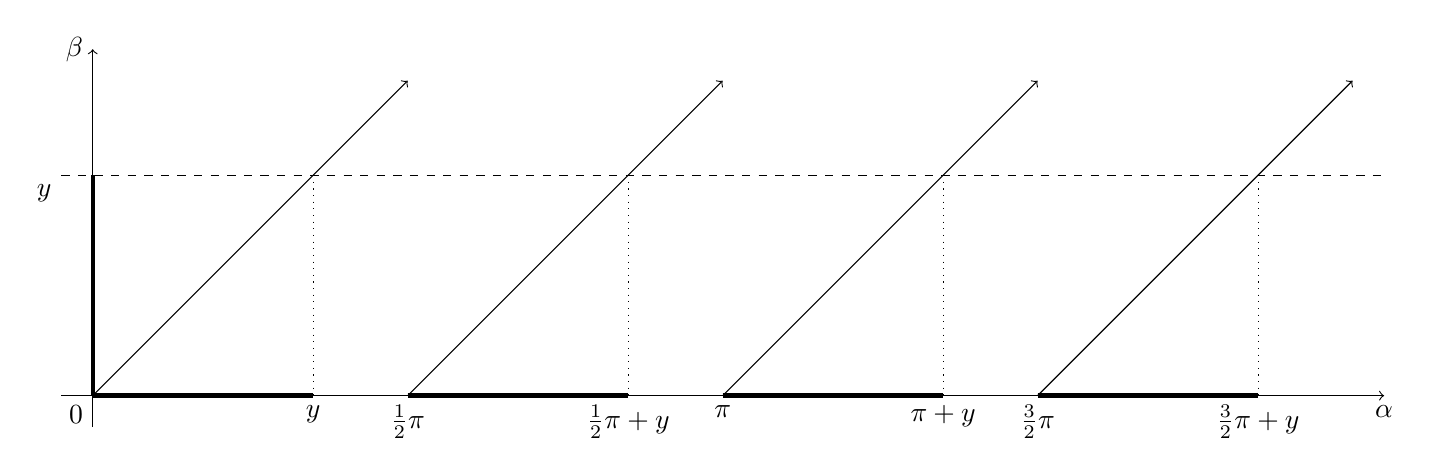
\begin{tikzpicture}[scale=4]
        % оси
        \draw [->] ( -0.1, 0 ) -- ( 4.1, 0 ) node [ below ] at ( 4.1, 0 ) {$\alpha$};
        \draw [->] ( 0, -0.1 ) -- ( 0, 1.1 ) node [ left ] at ( 0, 1.1 ) {$\beta$};

        % отрезок 1
        \draw [->] ( 0, 0 ) -- ( 1, 1 );
        \draw [dotted] ( 0.7, 0.7 ) -- ( 0.7, 0 );
        \draw [ultra thick] ( 0, 0 ) -- ( 0.7, 0 );
        \node [below left] ( 0, 0 ) {$0$};
        \node [ below ] at ( 0.7, 0 ) {$y$};
        % отрезок 2
        \draw [->] ( 1, 0 ) -- ( 2, 1 );
        \draw [dotted] ( 1.7, 0.7 ) -- ( 1.7, 0 );
        \draw [ultra thick] ( 1, 0 ) -- ( 1.7, 0 );
        \node [ below ] at ( 1, 0 ) {$\frac{1}{2}\pi$};
        \node [ below ] at ( 1.7, 0 ) {$\frac{1}{2}\pi + y$};
        % отрезок 3
        \draw [->] ( 2, 0 ) -- ( 3, 1 );
        \draw [dotted] ( 2.7, 0.7 ) -- ( 2.7, 0 );
        \draw [ultra thick] ( 2, 0 ) -- ( 2.7, 0 );
        \node [ below ] at ( 2, 0 ) {$\pi$};
        \node [ below ] at ( 2.7, 0 ) {$\pi + y$};
        % отрезок 4
        \draw [->] ( 3, 0 ) -- ( 4, 1 );
        \draw [dotted] ( 3.7, 0.7 ) -- ( 3.7, 0 );
        \draw [ultra thick] ( 3, 0 ) -- ( 3.7, 0 );
        \node [ below ] at ( 3, 0 ) {$\frac{3}{2}\pi$};
        \node [ below ] at ( 3.7, 0 ) {$\frac{3}{2}\pi + y$};

        % уровень y
        \draw [dashed] ( -0.1, 0.7 ) -- ( 4.1, 0.7 ) node [ below left ] at ( -0.1, 0.7 ) {$y$};
        \draw [ultra thick] ( 0, 0 ) -- ( 0, 0.7 );
    \end{tikzpicture}
    \caption{Преобразование угла $\alpha$ в угол $\beta$.}
\end{figure}

Функция распределения $F_\beta(y)$ угла $\beta$:
\begin{multline}
    F_\beta(y) = \probability{\beta < y}
    = \left \{
    \begin{array}{ll}
        0 ,                      & y < 0,                    \\
        \probability{\beta < y}, & 0 \le y < \frac{1}{2} \pi \\
        1,                       & \frac{1}{2} \pi \leq y
    \end{array}
    \right . = \\
    %
    = \left \{
    \begin{array}{ll}
        0 ,                                                                                                                                                                                                                                                                        & y < 0,                    \\
        \probability{\alpha \in \left [ 0, y \right )} + \probability{\alpha \in \left [ \frac{1}{2} \pi, \frac{1}{2} \pi + y \right )} + \probability{\alpha \in \left [ \pi, \pi + y \right )} + \probability{\alpha \in \left [ \frac{3}{2} \pi, \frac{3}{2} \pi + y \right )}, & 0 \le y < \frac{1}{2} \pi \\
        1,                                                                                                                                                                                                                                                                         & \frac{1}{2} \pi \leq y
    \end{array}
    \right . = \\
    %
    = \left \{
    \begin{array}{ll}
        0 ,                                               & y < 0,                    \\
        4 \probability{\alpha \in \left [ 0, y \right )}, & 0 \le y < \frac{1}{2} \pi \\
        1,                                                & \frac{1}{2} \pi \leq y
    \end{array}
    \right . = \\
    = \left \{
    \begin{array}{ll}
        0 ,            & y < 0,                    \\
        4 F_\alpha(y), & 0 \le y < \frac{1}{2} \pi \\
        1,             & \frac{1}{2} \pi \leq y
    \end{array}
    \right .
\end{multline}
Откуда функция плотности вероятности $f_\beta(y)$ величины $\beta$:
\begin{equation}
    f_\beta(y) = \derivative{y} F_\beta(y)
    = \left \{
    \begin{array}{ll}
        4 f_\alpha(y), & y \in \left [ 0, \frac{1}{2} \pi \right ),   \\
        0,             & y \notin \left [ 0, \frac{1}{2} \pi \right )
    \end{array}
    \right .
    = \left \{
    \begin{array}{ll}
        4 \frac{1}{2 \pi}, & y \in \left [ 0, \frac{1}{2} \pi \right ),   \\
        0,                 & y \notin \left [ 0, \frac{1}{2} \pi \right )
    \end{array}
    \right .
\end{equation}

Рассмотрим величину $\xi$:
\begin{equation}
    \xi = \tg \beta + \tg \left ( \frac{1}{2} \pi - \beta \right ) = \tg \beta + \ctg \beta
\end{equation}

Функция распределения $F_\xi(x)$ величины $\xi$:
\begin{multline}
    F_\xi(x)
    = \probability{\xi < x}
    = \probability{\tg \beta + \ctg \beta < x}
    = \probability{\frac{\sin \beta}{\cos \beta} + \frac{\cos \beta}{\sin \beta} < x} = \\
    %
    = \probability{\frac{\sin \beta \sin \beta + \cos \beta \cos \beta}{\cos \beta \sin \beta} - x < 0}
    = \probability{\frac{\sin^2 \beta + \cos^2 \beta - x \cos \beta \sin \beta}{\cos \beta \sin \beta} < 0} = \\
    %
    = \probability{\frac{1 - x \cos \beta \sin \beta}{\cos \beta \sin \beta} < 0}
    = \probability{\frac{1 - \frac{x}{2} \sin 2 \beta}{\cos \beta \sin \beta} < 0}
    = \probability{1 - \frac{x}{2} \sin 2 \beta < 0} = \\
    %
    = \probability{1 < \frac{x}{2} \sin 2 \beta}
    = \probability{2 < x \sin 2 \beta}
    = \left \{
    \begin{array}{ll}
        0,                                        & x < 2 , \\
        \probability{\frac{2}{x} < \sin 2 \beta}, & 2 \le x
    \end{array}
    \right . = \\
    %
    = \left \{
    \begin{array}{ll}
        0,                                                                                 & x < 2 , \\
        \probability{\arcsin \frac{2}{x} < 2 \beta < \frac{\pi}{2} - \arcsin \frac{2}{x}}, & 2 \le x
    \end{array}
    \right . = \\
    %
    = \left \{
    \begin{array}{ll}
        0,                                                                                                                        & x < 2 , \\
        \probability{\frac{1}{2} \arcsin \frac{2}{x} < \beta < \frac{1}{2} \left ( \frac{\pi}{2} - \arcsin \frac{2}{x} \right )}, & 2 \le x
    \end{array}
    \right . = \\
    %
    = \left \{
    \begin{array}{ll}
        0,                                                                                                                    & x < 2 , \\
        F_\beta(\frac{1}{2} \left ( \frac{\pi}{2} - \arcsin \frac{2}{x} \right )) - F_\beta(\frac{1}{2} \arcsin \frac{2}{x}), & 2 \le x
    \end{array}
    \right .
\end{multline}

Откуда плотность вероятности $f_\xi(x)$ величины $\xi$:
\begin{multline}
    f_\xi(x)
    = \derivative{x} F_\xi(x) = \\
    %
    = \left \{
    \begin{array}{ll}
        0,                                                                                                                                                                                                                                                                                                                                                                           & x < 2 , \\
        f_\beta \left ( \frac{1}{2} \left ( \frac{\pi}{2} - \arcsin \frac{2}{x} \right ) \right ) \left ( - \frac{1}{2} \frac{1}{\sqrt{ 1 - \left ( \frac{2}{x} \right )^2}} \left ( - \frac{2}{x^2} \right ) \right ) - f_\beta \left ( \frac{1}{2} \arcsin \frac{2}{x} \right ) \frac{1}{2} \frac{1}{\sqrt{ 1 - \left ( \frac{2}{x} \right )^2}} \left ( - \frac{2}{x^2} \right ), & 2 \le x
    \end{array}
    \right . = \\
    %
    = \left \{
    \begin{array}{ll}
        0,                                                                                                                                                                                                               & x < 2 , \\
        4 \frac{1}{2 \pi} \cdot \frac{1}{2} \frac{1}{\sqrt{ 1 - \left ( \frac{2}{x} \right )^2}} \frac{2}{x^2} + 4 \frac{1}{2 \pi} \cdot \frac{1}{2} \frac{1}{\sqrt{ 1 - \left ( \frac{2}{x} \right )^2}} \frac{2}{x^2}, & 2 \le x
    \end{array}
    \right . = \\
    %
    = \left \{
    \begin{array}{ll}
        0,                                                                                                              & x < 2 , \\
        2 \cdot 4 \frac{1}{2 \pi} \cdot \frac{1}{2} \frac{1}{\sqrt{ 1 - \left ( \frac{2}{x} \right )^2}} \frac{2}{x^2}, & 2 \le x
    \end{array}
    \right .
    %
    = \left \{
    \begin{array}{ll}
        0,                                                    & x < 2 , \\
        \frac{2}{\pi} \frac{x}{\sqrt{x^2 - 4}} \frac{2}{x^2}, & 2 \le x
    \end{array}
    \right . = \\
    %
    = \left \{
    \begin{array}{ll}
        0,                              & x < 2 , \\
        \frac{4}{\pi x \sqrt{x^2 - 4}}, & 2 \le x
    \end{array}
    \right .
    .
\end{multline}

\subsection*{Ответ:}
$
f_\xi(x)
= \left \{
\begin{array}{ll}
    0,                              & x < 2 ,   \\
    \frac{4}{\pi x \sqrt{x^2 - 4}}, & 2 \le x .
\end{array}
\right .
$

\section*{Задачи для самостоятельного решения}

Из раздела 18 сборника задач Ефимова и Поспелова.
\begin{enumerate}
    \item На занятии: 507.
    \item Дома: 498, 501, 505, 509, 510.
\end{enumerate}

Из сборника задач типового расчёта Чудесенко: 25, 26, 27, 28.